%----------------------------------------------------------------------------
\chapter{Implementation of the static fraud detection scenario}
%----------------------------------------------------------------------------

In this chapter the previously discussed financial fraud scenarios are implemented in 3 different graph database engines in static mode.
We cover the database engines, including their technical setup, query design, visual illustration capability, and implementation challenges.
In the end, all performance measurements are compared in the benchmark.

%----------------------------------------------------------------------------
\section{Neo4j}
%----------------------------------------------------------------------------

Neo4j is a Sweden-based graph database company developed graph database solutions that is widely used in popular companies like Walmart, Airbnb, Lyft, etc.
Its native query language is called Cypher and has an intuitive SQL-like syntax.
Cypher has a wide community, that makes find solutions online easier.
On the other hand, the documentation is well-structured and enables set up engine and write queries in a short period~\cite{robinson2015graph}.

Neo4j works with the \emph{labelled property graph model} and has the following components:

\begin{itemize}
  \item \textbf{Nodes} are the main data models connected with relationships and have labels and properties.
  \item \textbf{Relationships} describe the connection between nodes and have one or more attributes (properties).
  \item \textbf{Labels} act like classes for vertices in software engineering terms. Labels group the nodes by types and speed up the query.
  \item \textbf{Properties} define the attributes, \ie additional information about nodes or relationships. These attributes help to build a more detailed query.
\end{itemize}

Neo4j provides a web browser application, where user can import, monitor, and query data.
In this work, we used command-line tools to import the datasets faster and wrote queries in web applications.
All of the three fraud scenarios were turned into Cypher queries with a small effort.

\paragraph{Smurfing}

To detect the smurfing parent in the graph \texttt{User} node and \texttt{SENT\_TO} relationship is used for building the query.
Middleman players are collected in the 2nd line of \autoref{lst:smurfing_cypher} and filtered to be more than three instances.
The query returned 10 subgraphs, and 2 of them are shown in \autoref{fig:smurfing_output}.

\begin{lstlisting}[language=Cypher,frame=single,caption={Cypher smurfing query},label={lst:smurfing_cypher}]
MATCH (u1:User)-[t1:SENT_TO]->(pm:User)-[t2:SENT_TO]->(u2:User)
WITH u1 AS sender, u2 AS receiver, collect(pm) AS pms
  WHERE size(pms) >= 3
RETURN sender, receiver, pms
  LIMIT 10
\end{lstlisting}

\begin{figure}[!ht]
  \centering
  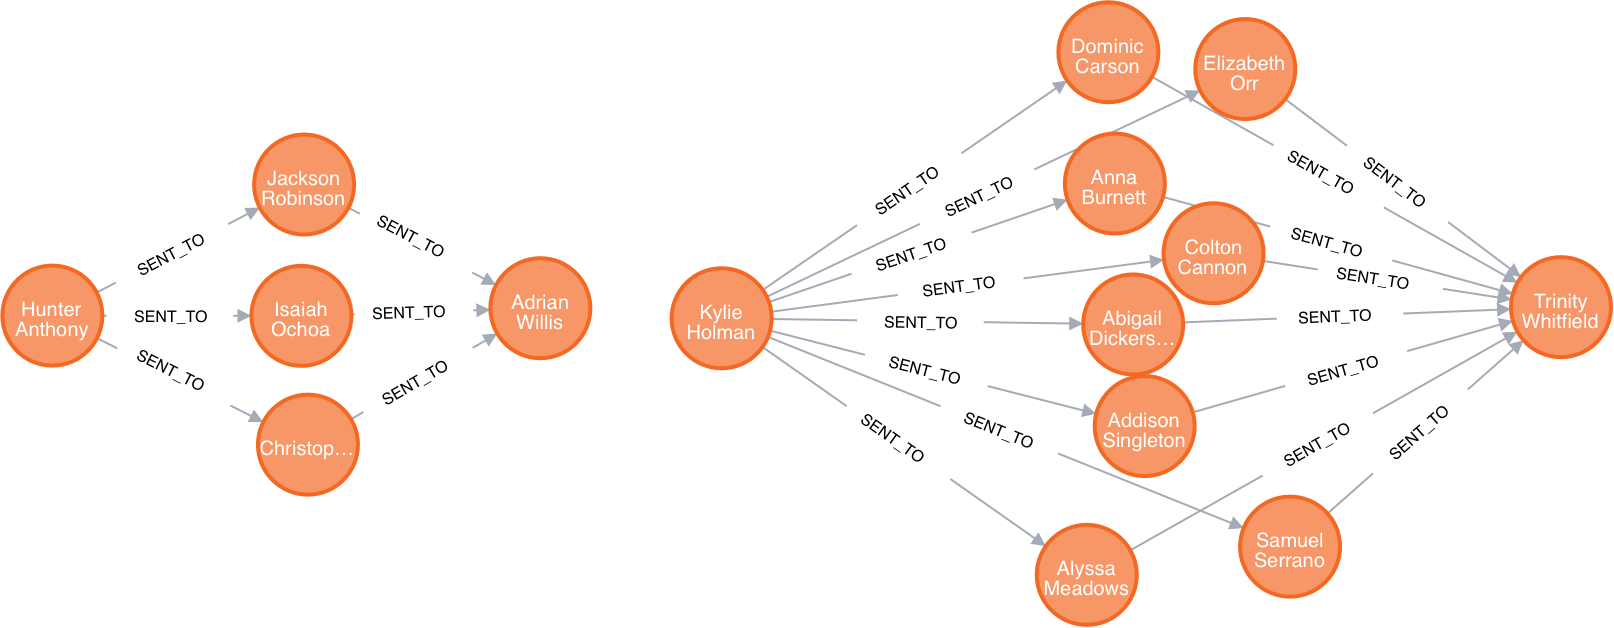
\includegraphics[width=\textwidth]{figures/smurfing_output.png}
  \caption{Smurfing query example result} 
  \label{fig:smurfing_output}
\end{figure}

\paragraph{Money laundering cycle}

Cycle detection is one of the primary use cases of graph engines.
In this work, we implemented a fixed-length cycle with a scenario where 4~middlemen participated in the fraud scheme.
The query is built with only one matching pattern in \autoref{lst:money_laundering_cypher}.
The 2 example out 10 subgraphs in \autoref{fig:money_laundering_cycle_output} visualize the result from the web application. 

\begin{lstlisting}[language=Cypher,frame=single,caption={Cypher money laundering cycle detection query},label={lst:money_laundering_cypher}]
MATCH (u1:User)-[:SENT_TO]->
  (m1:User)-[:SENT_TO]->
  (m2:User)-[:SENT_TO]->
  (m3:User)-[:SENT_TO]->
  (m4:User)-[:SENT_TO]->
  (u2:User)-[c:CONNECTED_TO]-(u1)
RETURN u1, m1, m2, m3, m4, u2, c
  LIMIT 10
\end{lstlisting}

\begin{figure}[!ht]
  \centering
  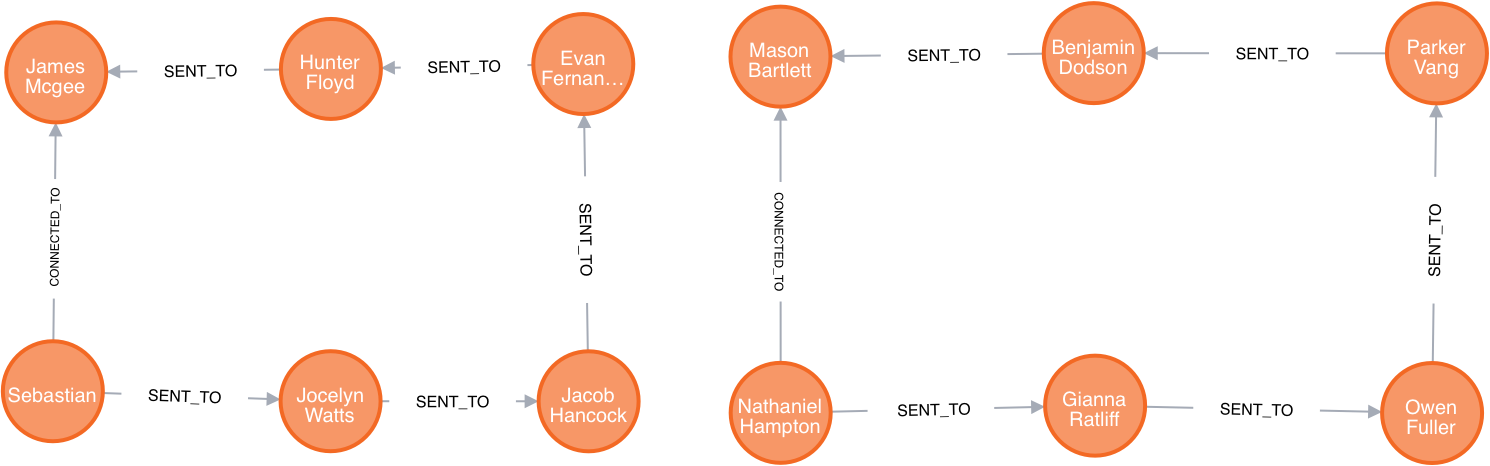
\includegraphics[width=\textwidth]{figures/cycle_output.png}
  \caption{Money laundering cycle query example result} 
  \label{fig:money_laundering_cycle_output}
\end{figure}

\paragraph{Biased reviews in e-commerce}

The most advanced query among these three scenarios is a biased review detection.
Firstly, the query collects the reviews by customers (\texttt{User} nodes) with constrained \texttt{Merchant} node and filter them with minimum limit size~4 in the 3rd line \autoref{lst:biased_reviews_cypher}.
Then customers with nearly perfect reviews (with more than 4 rating value) are filtered as a final result.
One of the detected subgraphs is matched with our query evaluation consists of two customers with seven perfect reviews(\autoref{fig:biased_reviews_output}).
The reviewed goods have \texttt{OWNED\_BY} relationships with a merchant name \textit{Klein} and marked as suspicious in comparison with others.

\begin{lstlisting}[language=Cypher,frame=single,caption={Cypher biased reviews detection query},label={lst:biased_reviews_cypher}]
MATCH (u:User)-[r:REVIEWED_TO]->(g:Good)-[o:OWNED_BY]->(m:Merchant)
WITH u, m, collect(r) as reviews, collect(g) as goods
  WHERE size(reviews) >= 4
UNWIND reviews as revList
WITH avg(revList.Rating) as avgRating, u, m, goods, reviews
  WHERE avgRating >= 4
RETURN u, m, goods, reviews
  LIMIT 10
\end{lstlisting}

\begin{figure}[!ht]
  \centering
  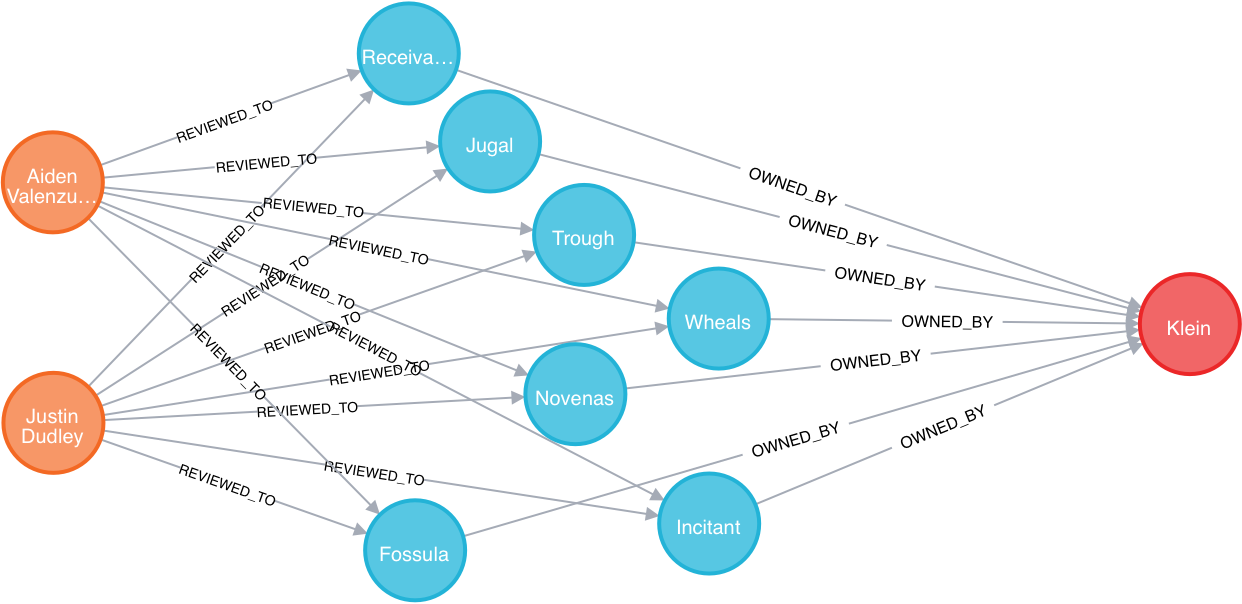
\includegraphics[width=\textwidth]{figures/biased_reviews_output.png}
  \caption{Biased reviews in e-commerce query example result} 
  \label{fig:biased_reviews_output}
\end{figure}

%----------------------------------------------------------------------------
\section{Oracle PGX}
%----------------------------------------------------------------------------

Oracle PGX~\cite{pgx_website} is a graph toolkit to implement ready algorithms or SQL-like pattern matching queries against the graph databases.
The engine can work in a single node or a distributed setup for large databases.
Data can be imported from several mediums with incremental update support.
In this work the flat CSV files are used for data seeding.
PGX shell is used to execute our queries during the experiment.
Oracle PGX works with a query language PGQL (Property Graph Query Language)~\cite{pgql_website} that supports both a SQL-like value-based constraints and topological constraints.

\paragraph{Smurfing}

Smurfing pattern matching query in PGQL is similar to the Cypher query.
The output variables are selected in the first command with \texttt{SELECT} keyword in PGQL (unlike in Cypher which usesr the \texttt{RETURN} keyword).

\begin{lstlisting}[language=Cypher,frame=single,caption={PGQL smurfing query},label={lst:smurfing_pgql}]
SELECT u.email, COUNT(u2), u3.email
MATCH (u:User)-[t:Transaction]-(u2:User)-[t2:Transaction]-(u3:User)
GROUP BY u, u3
HAVING COUNT(u2) > 3
\end{lstlisting}

\paragraph{Money laundering cycle}

The query to detect the money laundering cycle is also quite similar to the Cypher implementation.

\begin{lstlisting}[language=Cypher,frame=single,caption={PGQL money laundering cycle detection query},,label={lst:money_laundering_pgql}]
SELECT u1.email, m1.email, m2.email, m3.email, m4.email, u2.email
MATCH (u1:User)-[t:Transaction]-
  (m1:User)-[t2:Transaction]-(m2:User)-[t3:Transaction]-
  (m3:User)-[t4:Transaction]-(m4:User)-[t5:Transaction]-
  (u2:User)-[c:Connection]-(u1)
\end{lstlisting}

\paragraph{Biased reviews in e-commerce}

The biased reviews detection query is simpler and shorted than Cypher.
The 4th line in \autoref{lst:biased_reviews_pgql} illustrates the more optimized and convenient version of node groups access, which does not require several lines of data formatting.

\begin{lstlisting}[language=Cypher,frame=single,caption={PGQL biased reviews detection query},,label={lst:biased_reviews_pgql}]
SELECT u.email as customer, m.name as merchant, COUNT(r) as perfectreviews
MATCH (u:User)-[r:Review]-(g:Good)-[o:Ownership]-(m:Merchant)
GROUP BY u, m
HAVING COUNT(r) > 5 AND AVG(r.rating) = 5
\end{lstlisting}

%----------------------------------------------------------------------------
\section{TigerGraph}\label{sec:static_tigergrap_implementation}
%----------------------------------------------------------------------------

TigerGraph~\cite{tigergraph_website} is a native parallel graph database engine that supports a massively parallel computation model for queries and models.
The supported query language is called GSQL and designed to support a SQL-like syntax while allowing NoSQL developers to build Bulk-Synchronous Processing queries.
The query is built with loops and accumulators, which add extra complexity to design desired algorithm~\cite{DBLP:journals/corr/abs-1901-08248}.
Our implementation could not capture all the fraud scenarios completely, some of them left only return a subset of the desired outputs.

\paragraph{Smurfing}

In the smurfing scenario, it was only possible to return a single subgraph.
Due to the limitations of GSQL properties, sender and receiver node constrained queries are hard to design.
The parallel processing model allows only to apply independent parallel bulk processing.

\begin{lstlisting}[language=Cypher,frame=single,basicstyle=\footnotesize\ttfamily,caption=GSQL smurfing query]
CREATE QUERY findSmurfingUsers(int maxLimit) FOR GRAPH MyGraph syntax v2 {

  GroupByAccum<string senderName, SetAccum<string> middlemen> @middlemenAggregator;
  MaxAccum<string> @mostCommonSender;

  userRef = {User.*};
  receiver = SELECT tgt
    FROM
      userRef:sender - (Transaction>: t) - User:middleman - (Transaction>: t2)- User:tgt
    ACCUM
      tgt.@middlemenAggregator += (sender.name -> middleman.name),
      tgt.@mostCommonSender += sender.name
    HAVING tgt.@middlemenAggregator.get(tgt.@mostCommonSender).middlemen.size() >= 2
    LIMIT maxLimit;

  PRINT receiver [
    receiver.name,
    receiver.@mostCommonSender as sender,
    receiver.@middlemenAggregator.get(receiver.@mostCommonSender) as middlemen
  ];
}
\end{lstlisting}

\paragraph{Money laundering cycle}

We have successfully implemented the money laundering cycle query in GSQL but it performed slower than other systems.

\begin{lstlisting}[language=Cypher,frame=single,basicstyle=\footnotesize\ttfamily,caption=GSQL money laundering cycle detection query]
CREATE QUERY findMobileBankingFraud(int maxLimit) FOR GRAPH MyGraph syntax v2 {

  userRef = {User.*};

  senderList = SELECT snd
               FROM userRef:snd - (Transaction>*4.Connection) - User:tgt
               LIMIT maxLimit;

  PRINT senderList;
}
\end{lstlisting}

\paragraph{Biased reviews in e-commerce}

The biased reviews detection query in GSQL, only the merchant list was possible to return.
First, the customers are accumulated in the map type data structure with their review count and appearance frequency (lines between 11 and 13 in \autoref{lst:biased_reviews_gsql}).
Then merchants are filtered with the number of rating occurrences by the most active customer.

\begin{lstlisting}[language=Cypher,frame=single,basicstyle=\footnotesize\ttfamily,caption={GSQL biased reviews detection query},label={lst:biased_reviews_gsql}]
CREATE QUERY findBiasedReviews(int maxLimit) FOR GRAPH MyGraph syntax v2 {

  GroupByAccum<string customerId, SumAccum<int> ratingCount> @customerRatings;
  AvgAccum @rating;
  MaxAccum<string> @mostBiasedCustomer;

  merRef = {Merchant.*};

  merchants = SELECT m
              FROM  merRef:m - (<Ownership) - Good - (<Review:r) - User:u
              ACCUM m.@rating += r.rating,
                    m.@customerRatings += (u.name -> 1),
                    m.@mostBiasedCustomer += u.name
              HAVING m.@customerRatings.get(m.@mostBiasedCustomer).ratingCount > 4
              LIMIT maxLimit;

  PRINT merchants;
}
\end{lstlisting}

%----------------------------------------------------------------------------
\section{Benchmark} \label{sec:static_benchmark}
%----------------------------------------------------------------------------

We benchmarked the overall performance of the three graph database engines with two dataset sizes.
The benchmark was executed on a MacBook Pro 2015 laptop with an Intel Core i7 CPU and 16 GB RAM, using Java 11.0.6 JVM.

\paragraph{Small dataset}
In the small dataset \textit{``Smurfing''} and \textit{``Biased reviews''} queries are completed successfully in a reasonable amount of time (\autoref{fig:benchmark_small}).
\textit{``Money laundering cycle''} scenario challenged the systems, one of them -- TigerGraph failed to complete in a time limit.
TigerGraph engine has a time limit in query execution, which equals to 16 seconds.
In general, Neo4j performed very well in all scenarios.

\begin{figure}[!ht]
  \centering
  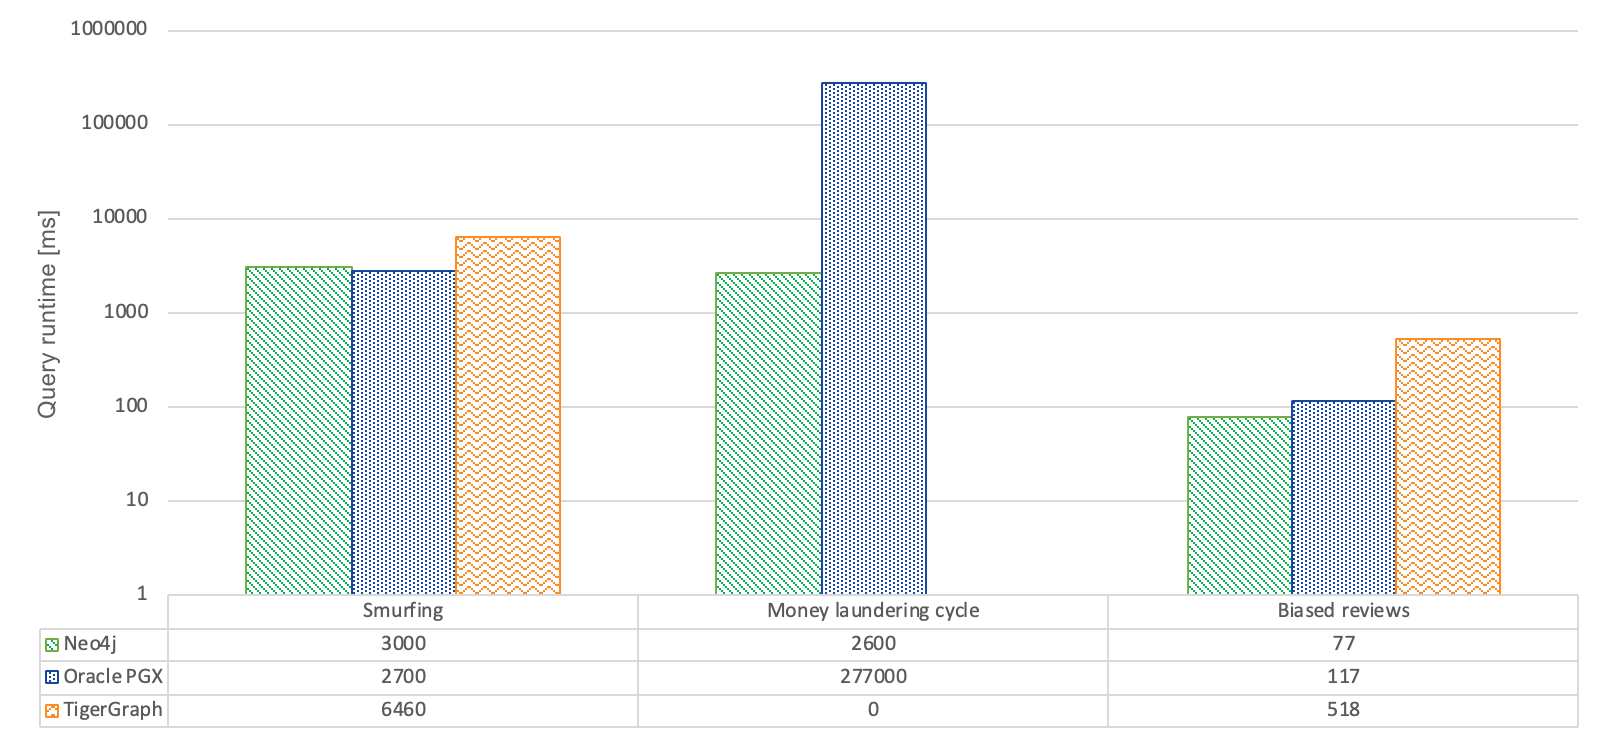
\includegraphics[width=\textwidth]{figures/static_benchmark_plot_small.png}
  \caption{Small dataset benchmark result} 
  \label{fig:benchmark_small}
\end{figure}

\paragraph{Large dataset}
In the large dataset, surprising findings are obtained from the benchmark (\autoref{fig:benchmark_large}).
\textit{``Smurfing''} fraud detection query has been evaluated successfully only by Neo4j in 116 seconds.
In the \textit{``Money laundering''} fraud case, Neo4j also failed to complete.
The last query, capturing the \textit{``Biased review''} scenario, ran quickly on all systems.
Oracle PGX performed best, $2\times$ and $6\times$ faster than Neo4j and TigerGraph, respectively.

\begin{figure}[!ht]
  \centering
  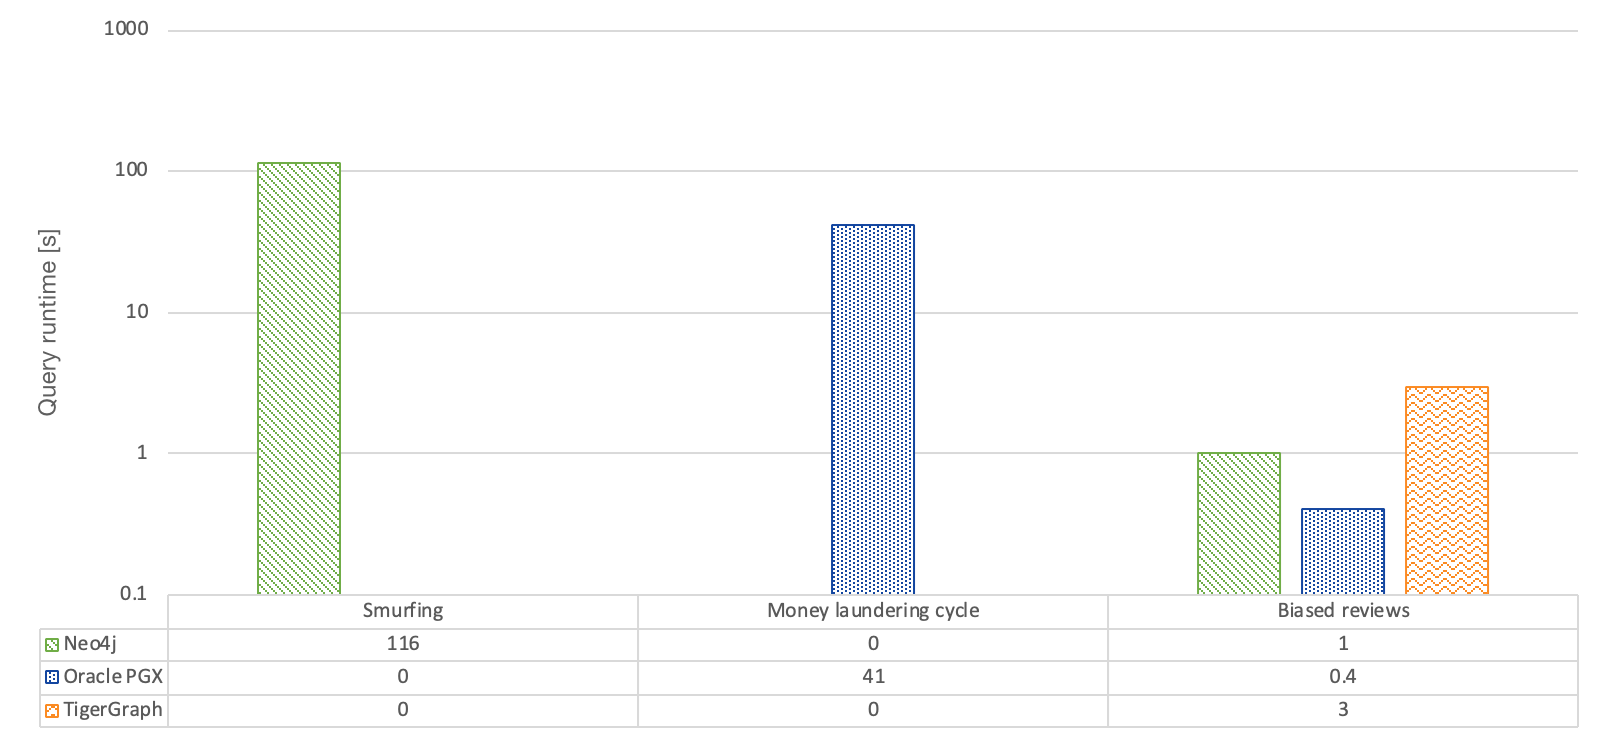
\includegraphics[width=\textwidth]{figures/static_benchmark_plot_large.png}
  \caption{Large dataset benchmark result} 
  \label{fig:benchmark_large}
\end{figure}
